\documentclass{beamer}

\usepackage{subfigure}
\usepackage{graphicx}
\usepackage{sidecap}
\usepackage{caption}
\usepackage{subcaption}
\captionsetup{compatibility=false}
\usepackage{appendixnumberbeamer}
\usepackage{amsmath}
% --
\usepackage{multirow}
\usepackage{xcolor}
\usepackage{setspace}
\usepackage{hyperref}
\usepackage{anyfontsize}

\beamertemplatenavigationsymbolsempty
\setbeamertemplate{footline}

\newenvironment{itemise} {\begin{itemize} \setlength{\itemsep}{0.2cm}} {\end{itemize}}
\usepackage[labelformat=empty]{caption}
\setbeamertemplate{sections/subsections in toc}[square]

%% COLORS
\definecolor{Gray}{gray}{0.9}
\definecolor{dblue}{rgb}{0.132,0.1,0.27}
\definecolor{mint}{cmyk}{1.0, 0.2, 0.6, 0.05}
\definecolor{ant}{cmyk}{0.5, 0.1, 0.0, 0.45}
\definecolor{lgray}{cmyk}{0.12, 0.0, 0.0, 0.17}
\definecolor{lred}{cmyk}{0.0, 0.9, 0.7, 0.0}


\usepackage{etoolbox}% http://ctan.org/pkg/etoolbox 
\usepackage{booktabs}

\newenvironment{literatur}{%
  \parskip2pt \parindent0pt \raggedright
  \def\lititem{\hangindent=0.5cm \hangafter1}}{%
  \par\ignorespaces}

\newcommand{\tb}[1]{{\color{blue}{\textbf{#1}}}}
\newcommand{\tm}[1]{{\color{mint}{\textbf{#1}}}}
\newcommand{\tr}[1]{{\color{red}{\textbf{#1}}}}
\newcommand{\tbs}[1]{{\color{blue}{#1}}}
\newcommand{\trs}[1]{{\color{red}{#1}}}
\newcommand{\tms}[1]{{\color{mint}{#1}}}
\newcommand{\tps}[1]{{\color{purple}{#1}}}
% Ilya: packages

\usepackage{tikz}
\usepackage{lmodern}
\usepackage{enumitem}

% Ilya: my commands

\newenvironment{mytemize}
{\vfill\itemize[nolistsep,itemsep=\fill,label=\color{blue}{$\triangleright$}]}
  {\enditemize}


\newenvironment{mynumerate}
{\vfill\enumerate[nolistsep,itemsep=\fill,label=\arabic*.]}
  {\endenumerate}

\newcommand{\hitem}[1]{
  {\color{blue}{$\triangleright$}} 
  {#1} 
  {\hfill}
}

\setlist[itemize]{label= \color{blue}{$\triangleright$}}
\setlist[enumerate]{label = \arabic*.}

\newcommand{\rarr}{$\Rightarrow$\ }



%\href{<Ziel>}{<Eingefasster Text>} 

%\logo{\includegraphics[height=0.7cm]{BdFlogo.eps}\hspace{300pt}\vspace{-5pt}}
%\logo{\includegraphics[height=0.8cm]{BdFlogo.eps}}
%\logo{\pgfputat{\pgfxy(-6.2,-0.5)}{\pgfbox[center,base]{\includegraphics[height=0.8cm]{BdFlogo.eps}}}}

%------------------------------------------------------------------------------------
% TITLE
%------------------------------------------------------------------------------------
\title[PSME]{Macroeconomics\\ Lecture 8 -- RBC in Closed Economy II} 
\author[I. Eryzhenskiy]{Ilya Eryzhenskiy}
\institute[BdF]{PSME Panth\'{e}on-Sorbonne Master in Economics}
\date[PSME macro]{Fall 2023}

%---BEGIN------------------------------------------------------------------------------
\begin{document}

\begin{frame}
  \maketitle
\end{frame}

\begin{frame}{Overview}
  \tableofcontents
\end{frame}

\section{Solution techniques}
%---FRAME------------------------------------------------------------------------------
\begin{frame}
\frametitle{Outline}
\tableofcontents[currentsection]
\end{frame}
%---FRAME------------------------------------------------------------------------------
\begin{frame}{Previously on RBC...}
We have boiled down the baseline RBC model to 4 equations: 
    \begin{align*}
\frac{v'(1-N_t)}{u'(C_t)}&= A_t F'_N(K_t,N_t) \nonumber\\
u'(C_t) &= \beta E_t [u'(C_{t+1})(A_{t+1} F'_K(K_{t+1},N_{t+1})+1-\delta)] \\
C_t+K_{t+1}-(1-\delta)K_{t} &= A_t F(K_t,N_t) \nonumber \\
\ln A_t &= \rho \ln A_{t-1} + \varepsilon_t
\end{align*}

Hard system to solve --  help from the computer is needed \vfill
But first, choose $u(\cdot), v(\cdot), F(\cdot, \cdot)$ and:
\begin{enumerate}
    \item Solve for \tb{steady state} (usually easy -- see below) 
    \item Find \tb{linear approximation around steady state} (a lot of calculus, programs like \texttt{gEcon.py} can do it for basic models like this one) 
    \item Decide how you choose \tb{parameter values}
\end{enumerate}

\end{frame}


%---FRAME------------------------------------------------------------------------------
\begin{frame}{Choosing functional forms}

Let's look at solution with typical functions:
  \begin{mytemize}
\item \textbf{Preferences} -- we will use $u(C_t) - \nu (\underset{+}{N_t})$ instead of $u(C_t)+v(\underset{+}{1-N_t})$ \tms{($\nu$ is "nu", it is not $v$)}:
\begin{align*}
  u(C_t) -  \nu (N_t) = \ln C_t 
  - \chi \frac{N_t^{1+\eta}}{1+\eta},
\end{align*}
$\eta$ ("eta") is the inverse of elasticity of labor supply for given consumption level. $\chi$ measures how strong is disutility of labor
\item \textbf{Production function} --  the \tb{Cobb-Douglas} function:
\begin{align*}
  Y_t = A_t F(K_t, N_t) = A_t K_t^{\alpha}N_t^{1-\alpha},
\end{align*}
where $\alpha$ is share of capital income in total income
\end{mytemize}

\end{frame}

\begin{frame}{Cobb-Douglas and income shares}
    By manupulating firm FOC's we get that $\alpha$ is share of capital in total income (GDP) and $1-\alpha$ is the share of labor income: 
      \begin{align*}
	\alpha A_t K_t^{\alpha-1} N_t^{1-\alpha} &= R_t \Leftrightarrow \alpha A_t K_t^{\alpha-1} N_t^{1-\alpha}K_t  = R_t K_t \Leftrightarrow \\ 
	\alpha A_t K_t^{\alpha} N_t^{1-\alpha} &= R_t K_t \Leftrightarrow \alpha Y_t = R_t K_t \Leftrightarrow \trs{\alpha = \frac{R_t K_t}{Y_t}}  
 \end{align*}
 \begin{align*}
 (1-\alpha)A_t K_t^{\alpha}N_t^{-\alpha} &= w_t \Leftrightarrow (1-\alpha)A_t K_t^{\alpha}N_t^{-\alpha} N_t = w_t N_t \Leftrightarrow\\
 (1-\alpha)A_t K_t^{\alpha}N_t^{1-\alpha} &= w_t N_t \Leftrightarrow (1-\alpha)Y_t = w_t N_t \Leftrightarrow \trs{1-\alpha = \frac{w_t N_t}{Y_t}}
\end{align*}
\end{frame}
%---FRAME------------------------------------------------------------------------------
\begin{frame}{First Order Conditions with chosen functions}
\textbf{Consumption-labor}:
\begin{equation*}
\frac{\nu'(N_t)}{u'(C_t)}= w_t \Leftrightarrow \chi N_t^\eta C_t=w_t 
\end{equation*}
\textbf{Euler equation}, \textbf{optimal capital holding}:
\begin{align*}
u'(C_t) = \beta E_t u'(C_{t+1})(1+r_t) &\Leftrightarrow
  \frac{1}{C_t} =  \beta  E_t \left[\frac{1}{C_{t+1}}\right](1+r_t) \\
u'(C_t) = \beta E_t [u'(C_{t+1})(R_{t+1}+1-&\delta)] \Leftrightarrow \frac{1}{C_t} =  \beta  E_t \left[\frac{R_{t+1} + 1 - \delta}{C_{t+1}}\right]
\end{align*}
\vfill

Firms' \textbf{capital and labor optimality}: 
  \begin{align*}
	\alpha A_t K_t^{\alpha-1} N_t^{1-\alpha} &= R_t\\ (1-\alpha)A_t K_t^{\alpha}N_t^{-\alpha} &= w_t
\end{align*}

\textbf{Resource constraint}:
\begin{align*}
  C_t+K_{t+1}-(1-\delta)K_t= A_t K_t^\alpha N_t^{1-\alpha} 
\end{align*}
\end{frame}
%---FRAME------------------------------------------------------------------------------
\begin{frame}{Steady state: definition}
In the steady state:
\begin{enumerate}
    \item No shocks happen -- set shock variables to 0
    \item All variables are constant -- write time index $ss$ (or any other notation) instead of $t, t+1 ...$
\end{enumerate}
\vfill
    Steady-state TFP must be equal to 1:
    \begin{align*}
        \ln A_{ss} = \rho \ln A_{ss} + \underbrace{\varepsilon_t}_{=0}\Leftrightarrow \ln A_{ss} = \rho \ln A_{ss} \\
        \Leftrightarrow (1-\rho) \ln A_{ss} = 0 \Leftrightarrow \ln A_{ss} = 0 \Leftrightarrow A_{ss} = 1 
    \end{align*}
    \vfill
    Another simple result is \textbf{steady-state investment that only replaces depreciated capital}: 
    $$K_{ss} = (1-\delta)K_{ss} + I_{ss} \Leftrightarrow I_{ss} = \delta K_{ss}$$
\end{frame}

\begin{frame}{Steady state -- First Order Conditions}
\textbf{Consumption-labor}:
\begin{equation*}
\chi N_{ss}^\eta C_{ss} = w_{ss}
\end{equation*}
\textbf{Euler equation}, \textbf{optimal capital holding}:
\begin{align*}
  \frac{1}{C_{ss}} =  \beta  \frac{1}{C_{ss}}(1+r_{ss}) &\Leftrightarrow \textcolor{red}{1 = \beta (1+r_{ss})} \\
 \frac{1}{C_{ss}} =  \beta  \frac{R_{ss} + 1 - \delta}{C_{ss}} &\Leftrightarrow \textcolor{red}{1 = \beta(R_{ss} + 1 - \delta)}
\end{align*}
\vfill

Firms' \textbf{capital and labor optimality}: 
  \begin{align*}
	K_{ss}^{\alpha-1} N_{ss}^{1-\alpha} &= R_{ss}\\ (1-\alpha) K_{ss}^{\alpha}N_{ss}^{-\alpha} &= w_{ss} 
\end{align*}

\textbf{Resource constraint}:
\begin{align*}
  C_{ss}+\delta K_{ss}=  K_{ss}^\alpha N_{ss}^{1-\alpha} 
\end{align*}

\end{frame}
%---FRAME------------------------------------------------------------------------------

\begin{frame}{Make the model linear: why and how}
Behavior of a non-linear system of many variables is an advanced problem, even for computers \\ \vfill 
    We are most interested in a simpler problem: the behavior of the economy \textbf{around the steady state} \\ \vfill
    That is, we assume that business cycles are relatively small. Cannot study \textbf{deep recessions} with linearized RBC 
    \\ \vfill
    When we look at \textbf{local} behaviour of a dynamic system, functions are nearly linear -- think of Taylor expansion \\ \vfill
    Two main ways of linearization are Taylor expansion of model equations and log-linearization
\end{frame}

\begin{frame}{Log-linearization of equations}
  Log-linearization -- most widespread linearization technique in macro literature \\ \vfill
  Gives percentage deviations from s.s. value \tms{(like percentage deviations from trend, Lec. 6)}
  \vfill
  Substitution rules for each variable $x_t$: 
  $$x_t = x_{ss} e^{\tilde x_t}, \quad \text{with} \quad \tilde x_t \equiv \ln x_t - \ln x_{ss}$$ 
  \vfill
  Then, the following approximations are used:
  \begin{enumerate}
	\item $e^{\tilde x_t} \approx 1 + \tilde x_t$ ($\Leftrightarrow \ \ln (1+\tilde x_t) \approx \tilde x_t$)
	\item $\tilde x_t \tilde y_t \approx 0$  (we are doing a \textbf{first-order} approximation) 
  \end{enumerate}

\end{frame}

\begin{frame}{Log-linearized model}
Some equations (like consumption-labor and firm FOCs) are easily linearized, other require more work:
  \begin{align*}
	  \tilde C_t + \eta \tilde N_t &=  \tilde w_t \\
	 \tilde C_{t} &= E_t \left[ \tilde C_{t+1} -  \beta R_{ss} \tilde R_{t+1}\right]  \\
	  \tilde A_t + (\alpha -1) \tilde K_t + (1-\alpha) \tilde N_t &= \tilde R_t \\
	  \tilde A_t + \alpha \tilde K_t -\alpha \tilde N_t &= \tilde w_t \\
	  C_{ss} \tilde C_t + K_{ss} (\tilde K_{t+1} - (1-\delta) \tilde K_t) &= K_{ss}^\alpha L_{ss}^{1-\alpha}(\tilde A_t + \alpha \tilde K_t + (1-\alpha) \tilde N_t) \\
	  \tilde A_{t+1} &= \rho \tilde A_t + \varepsilon_t
  \end{align*}

  A system of linear equations \rarr let's write it in \tb{state space} form
\end{frame}
\begin{frame}{Numerical solution: linear state space}

First, group the variables to write the state-space system as:
  \begin{align*}
	\begin{bmatrix}x^p_{t+1} \\ E_t x^j_{t+1}\end{bmatrix} &= A \begin{bmatrix}x^p_{t} \\ x^j_{t}\end{bmatrix} + R \nu_{t+1} \\
 y_t &= G \begin{bmatrix}x^p_{t} \\ x^j_{t}\end{bmatrix}
  \end{align*}
  with $x^p_t$ the vector of \tb{pre-determined variables}, $x^j_t$ the vector of \tb{jump variables}, $\nu_t$ is vector of shocks and $y_t$ are all the remaining \tb{static variables} that can be computed from $x^p_t, x^j_t$  \vfill

  Pre-determined variables are determined by their \textbf{past values}: in RBC, they are $K_t, A_t$ \vfill
  Jump variables are determined \textbf{looking in the future}: in RBC, it is $C_t$ \vfill
  The only shock we considered is the TFP shock $\varepsilon_t$ \\
  The remaining variables are static: $N_t, w_t, r_t, R_t, Y_t, I_t...$
  
  \end{frame}

  \begin{frame}{RBC as linear state space}
  Pre-determined vector $x^p_t = [A_t\ K_t]'$, jump vector $x^j_t = C_t$, shock vector $\nu_t = [\varepsilon_t\ 0\ 0]'$
  \begin{align*}
	\begin{bmatrix}\tilde K_{t+1} \\ 
 \tilde A_{t+1} \\
 E_t \tilde C_{t+1}\end{bmatrix} &= A \begin{bmatrix}\tilde K_{t} \\ \tilde A_t \\ \tilde C_t \end{bmatrix} + R \begin{bmatrix}\varepsilon_{t} \\ 0 \\ 0 \end{bmatrix} \\
 \begin{bmatrix} \tilde N_{t} \\ \tilde  w_{t} \\ \tilde r_t \\ \tilde R_t \\ \tilde Y_t \\ \tilde I_t \end{bmatrix} &= G \begin{bmatrix}\tilde K_{t} \\ \tilde A_t \\ \tilde C_t\end{bmatrix}
  \end{align*}
  \end{frame}

  \begin{frame}{Blanchard-Kahn condition}
Matrix $A$ consists of expressions of model parameters. When parameters are set (we discuss below how it can be done), the computer can:
\begin{mynumerate}
\item Find eigenvalues and eigenvectors of the $A$ matrix
\item Check that number of \textbf{unstable} eigenvalues (absolute value $\geq 1$) is same as number of jump variables -- the \tb{Blanchard-Kahn condition}
%\item Find the path of convergence to steady state for any initial state 
\end{mynumerate}
\vfill
If (and only if) the condition is met, there is exactly one way for the economy to converge to the steady state. This will be the dynamic equilibrium 
\end{frame}
\section{Parameter values: calibration vs. estimation}
\begin{frame}
\frametitle{Outline}
\tableofcontents[currentsection]
\end{frame}
\begin{frame}{Feeding numbers to models}

How to choose parameter values? Several approaches for RBC and any \tb{DSGE} (Dynamic Stochastic General Equilibrium) model:
\begin{mynumerate}
\item Setting values from established macro literature 
  \begin{mytemize}
  \item example: $\alpha = 1/3$ (share of capital income in GDP)
  \item how to know what is ``established''? Find $>2$ papers in high-rank journals or working papers of institutions such as NBER, IMF, ECB... 
  \end{mytemize}
\item \tb{Calibration} $\rightarrow$ picking parameter values by hand to match some empirical \tb{target}, often about \textbf{steady state} 
  \begin{mytemize}
  \item Example: labor disutility $\chi$ such that $N_{ss} = 1/3$, historical value from U.S. statistics
  \end{mytemize}
\end{mynumerate} 
\vfill
  Can \textbf{match moments} in a more disciplined way: General Method of Moments (GMM) $\to$ \tb{estimation} method
\end{frame}
\begin{frame}{Model and data}
\begin{enumerate}
  \item[3.] \tb{Estimation} $\rightarrow$ automated \textbf{econometric} procedures; not covered in lectures, separate course needed. \\ 2 main classes of methods: 
  \begin{mytemize}
  \item \underline{Frequentist}: Rely on relationships between theoretical probabilities and empirical frequencies \\ Uses OLS, GMM, \tb{Maximum Likelihood}, \tb{Kalman filter}  
  \item \underline{Bayesian}: Rely on probabilities as \textbf{beliefs} of researcher; use data and Bayes rule to update prior beliefs (priors) to posterior beliefs (posteriors). \\ Uses Maximum Likelihood, Kalman filter, Monte Carlo Markov Chains
  \end{mytemize}
\end{enumerate}
\vfill
  Will look at \textbf{calibrated} models in lectures; estimation is left for TD. Ready-to-use python functions will implement a mix of frequentist and Bayesian method: Maximum Aposteriori (MAP) estimation
\end{frame}
  
\begin{frame}
  \begin{figure}[ht]
	
\includegraphics[width = 0.8\linewidth]{FIGURES/new_method_meme.png}
	\centering
	\caption{A representation of how you will feel doing model estimation (it's okay)}
  \end{figure}
\end{frame}
\begin{frame}{Calibration}

\begin{center}

\begin{tabular}{c c c c c c c} 
\toprule
$\beta$ & $\alpha$ & $\eta$ & $\chi$ & $\delta$ & $\rho$ \\ 
\hline 
0.99 & 0.33 & 1 & 8 & 0.025 & 0.8 \\ 
\bottomrule
\end{tabular} 
\end{center}
\vfill
Values established in RBC literature:
\begin{mytemize}
\item  $\alpha=1/3$ in Cobb-Douglas production function: long-run (historical) capital share in national income in US
\item Capital depreciation rate is 10\% annually \rarr $2.5\%$ quarterly $\delta=0.025$
\item $\rho$ must be high (can reach $0.99$, but never 1) for high business cycle persistence: see King \& Rebelo paper
\end{mytemize}
\vfill
Values calibrated to match a \tb{target}:
\begin{mytemize}
\item discount factor $\beta$ to yield real \textit{annual} interest rate of $4\%$ (quarterly interest $\approx 1\%$)\rarr $\beta = 1/(1+r_{ss})=1/(1+0.04/4)\approx 0.99$ 
\item labor disutility $\chi$ such that $N_{ss} = 1/3$, historical value from U.S. statistics
\end{mytemize}

\end{frame}

\section{Model outputs}
%---FRAME------------------------------------------------------------------------------
\begin{frame}
\frametitle{Outline}
\tableofcontents[currentsection]
\end{frame}
%---FRAME------------------------------------------------------------------------------
%---FRAME------------------------------------------------------------------------------
\begin{frame}{Stochastic simulation -- an example}

\begin{center}
%{\small
%Figure. 
%}
\vspace{-5mm}
\begin{figure}[h!]
  \subfigure{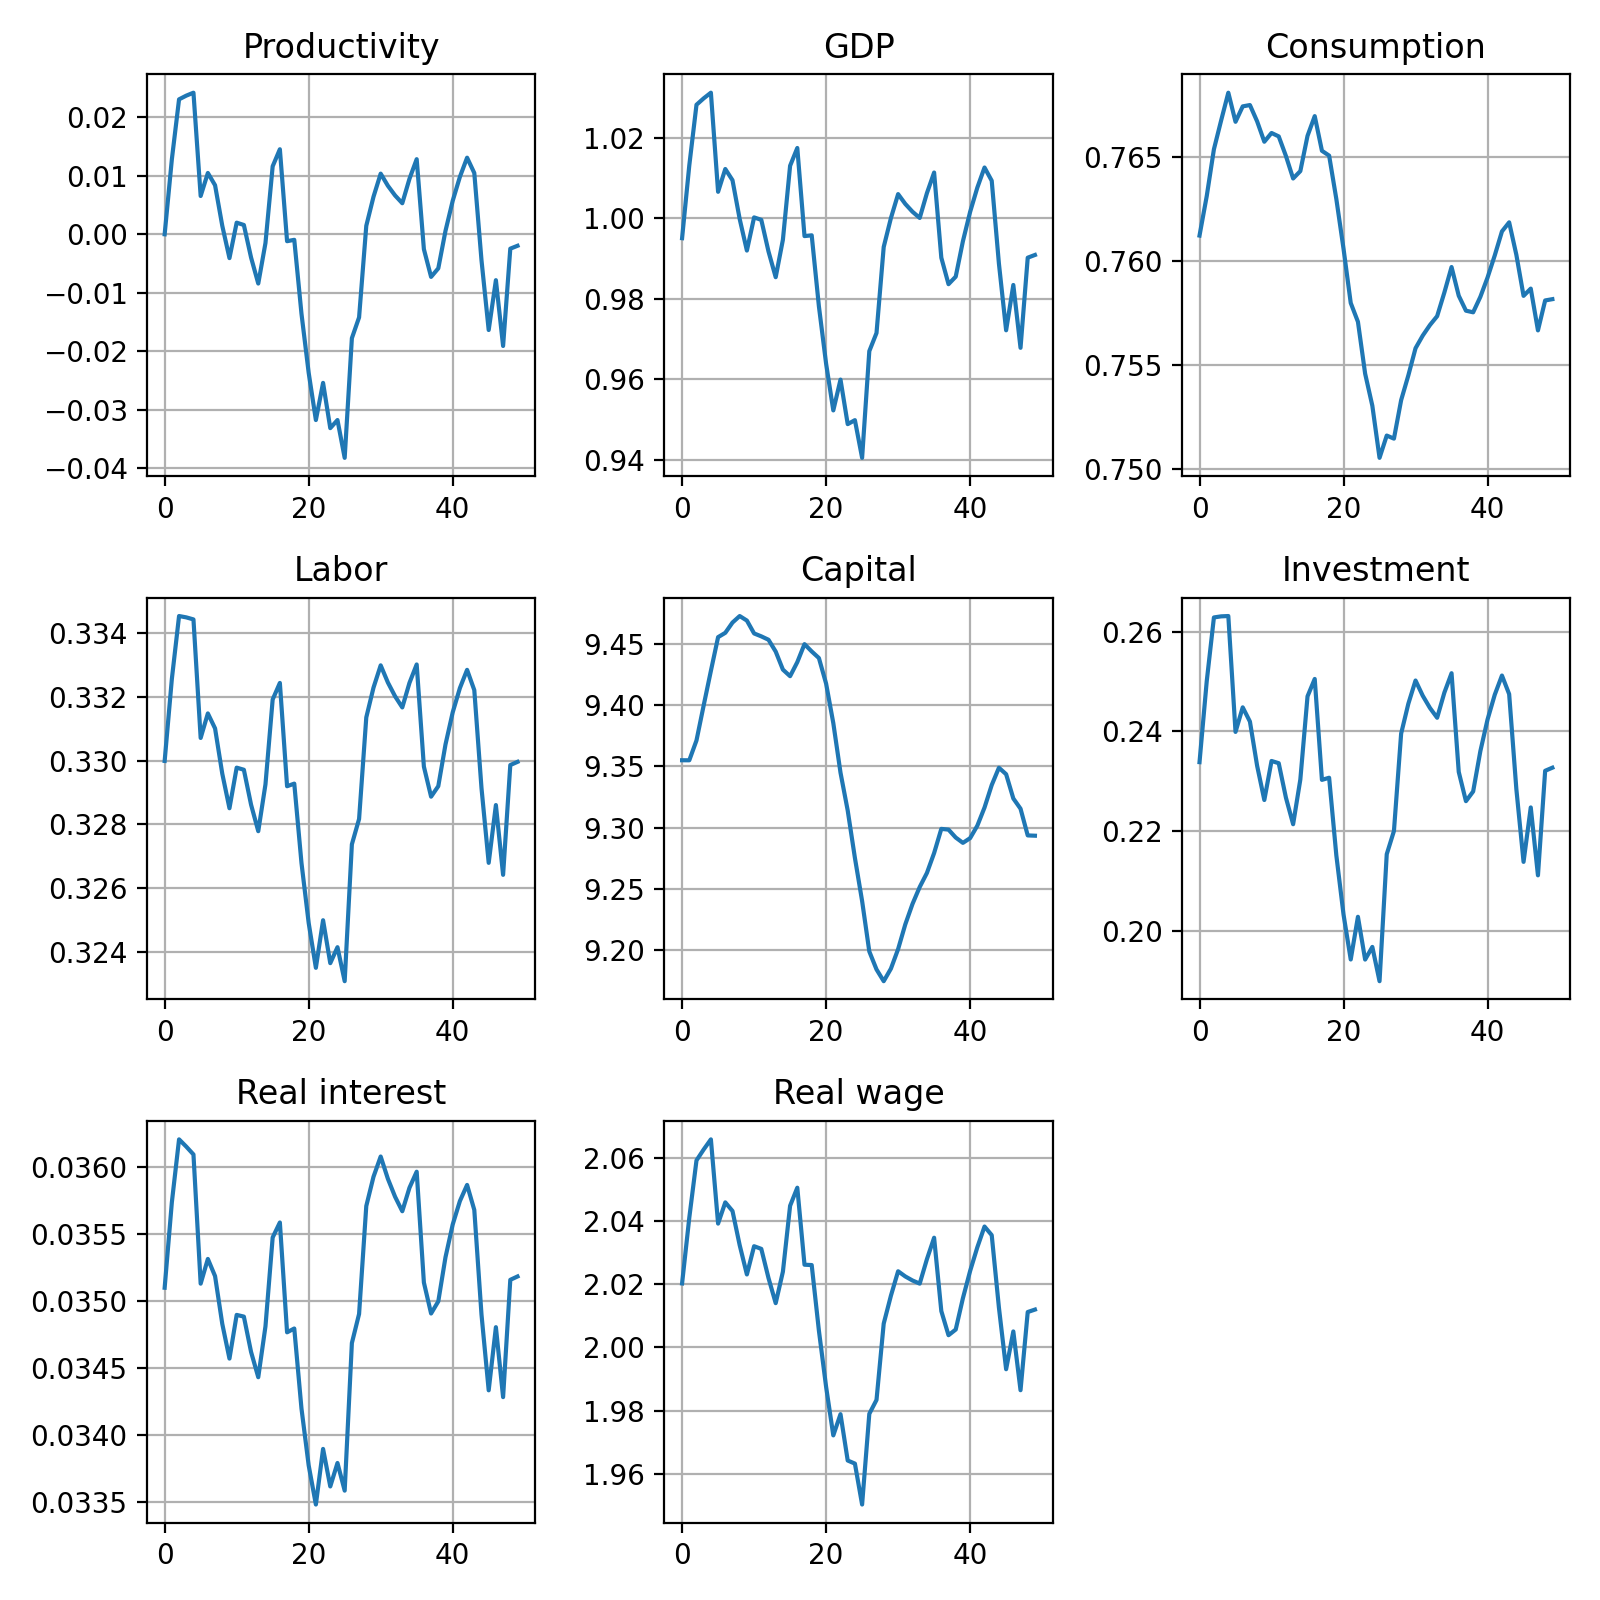
\includegraphics[trim=0 0 0 0,clip,width=0.75\textwidth]{FIGURES/rbc_stochsim8.png}
	}      
	%\subfigure{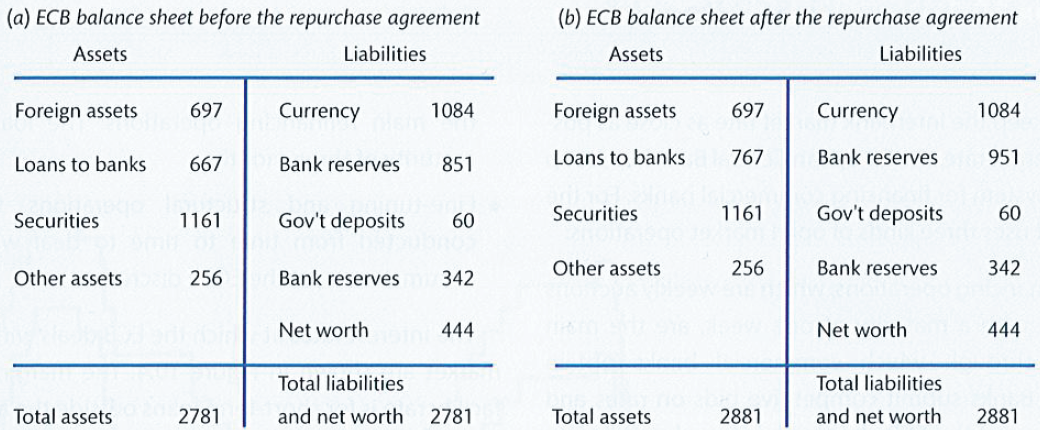
\includegraphics[trim=0 00 0 00,clip,width=0.6\textwidth]{FIGURES/5_CB_balance_sheet_OMO}
	%} 	
	%[trim=left bottom right top
\end{figure}
%\vspace{-2mm}
%\begin{minipage}{0.5\columnwidth}
%\tiny	
%\textbf{Source.} Burda and Wyplosz (2017), Figure 14.1.\\
%\end{minipage}
\end{center}
\vspace{-5mm}
\small
\tr{Attention:} here and henceforth model linearized, not \textbf{log-}linearized by computer \rarr variables in \textbf{levels}, not \textbf{relative deviations} from s.s.
\end{frame}

\begin{frame}{Stochastic simulation -- 1000 examples}

  We simply run the above simulation 1000 times. \textbf{Sequence of shocks is different every time} \rarr dynamics different. Interest and wages not plotted.
\begin{center}
%{\small
%Figure. 
%}
\vspace{-5mm}
\begin{figure}[h!]
  \subfigure{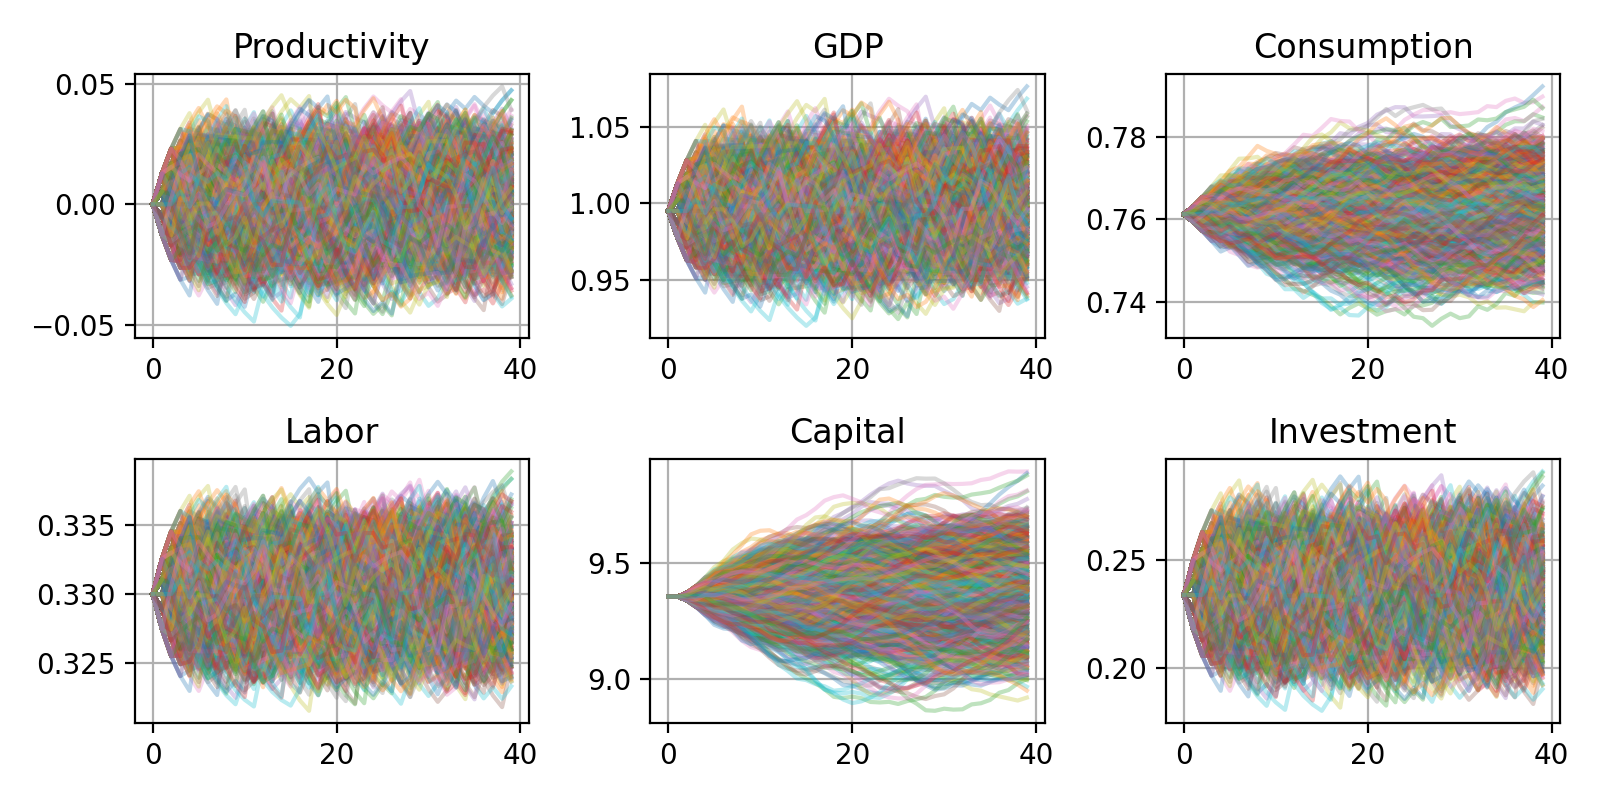
\includegraphics[trim=0 0 0 0,clip,width=0.98\textwidth]{FIGURES/rbc_spaghetti.png}
	}      
	%\subfigure{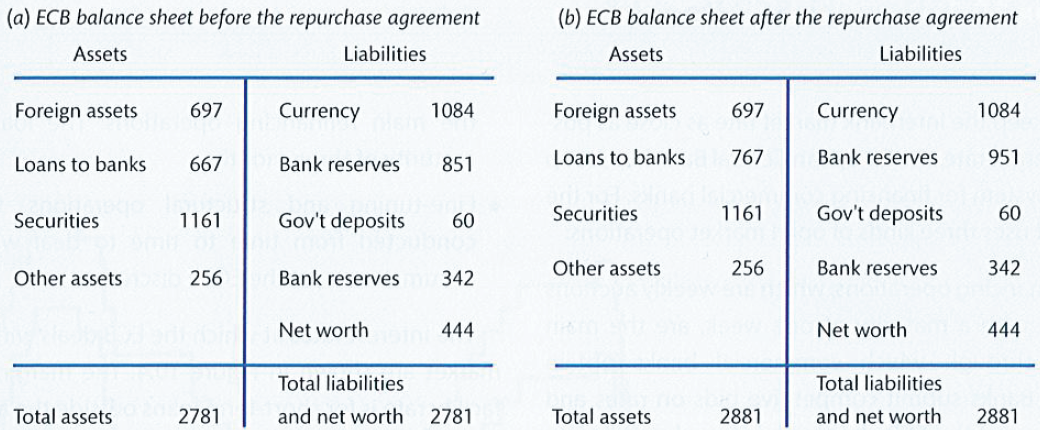
\includegraphics[trim=0 00 0 00,clip,width=0.6\textwidth]{FIGURES/5_CB_balance_sheet_OMO}
	%} 	
	%[trim=left bottom right top
\end{figure}
%\vspace{-2mm}
%\begin{minipage}{0.5\columnwidth}
%\tiny	
%\textbf{Source.} Burda and Wyplosz (2017), Figure 14.1.\\
%\end{minipage}
\end{center}

\end{frame}

%\begin{frame}{Model variances vs. empirical variances}
%  Compare average standard deviations of 3 variables: GDP, consumption, investment: $\sigma_Y, \sigma_C, \sigma_I$.
%  \vfill 
%  Model results using 1000 simulations: 
%  \begin{mynumerate}
%  \item $\frac{\sigma_C}{\sigma_Y} = 0.15$ 
%  \item $\frac{\sigma_I}{\sigma Y} = 4.5$ 
%  \end{mynumerate}
%  \vfill
%  Same statistics in de-trended US data (King\& Rebelo):
%  \begin{mynumerate}
%  \item $\frac{\sigma_C}{\sigma_Y} = 0.74$ 
%  \item $\frac{\sigma_C}{\sigma_Y} = 2.9$ 
%  \end{mynumerate}
% \vfill 
%  Our model exaggerates the difference in variances, but \textbf{reproduces the pattern}: $\sigma_C < \sigma_Y < \sigma_I$ \\
%
%\end{frame}

%---FRAME------------------------------------------------------------------------------
\begin{frame}{Impulse response functions --- A, Y}

  Transitory TFP shock: $\varepsilon$ rises from 0 to 0.1 ($=\sigma_\epsilon$) at $t=2$ and is at 0 afterwards:
\begin{center}
%{\small
%Figure. 
%}
\vspace{-5mm}
\begin{figure}[h!]
  \subfigure{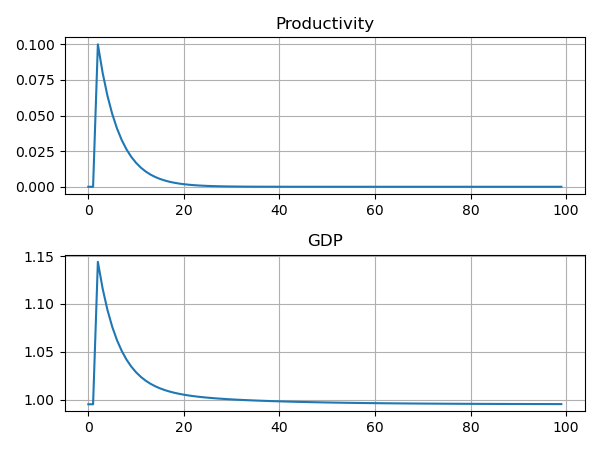
\includegraphics[trim=0 0 0 0,clip,width=0.9\textwidth]{FIGURES/irf_z_y.png}
	}      
	%\subfigure{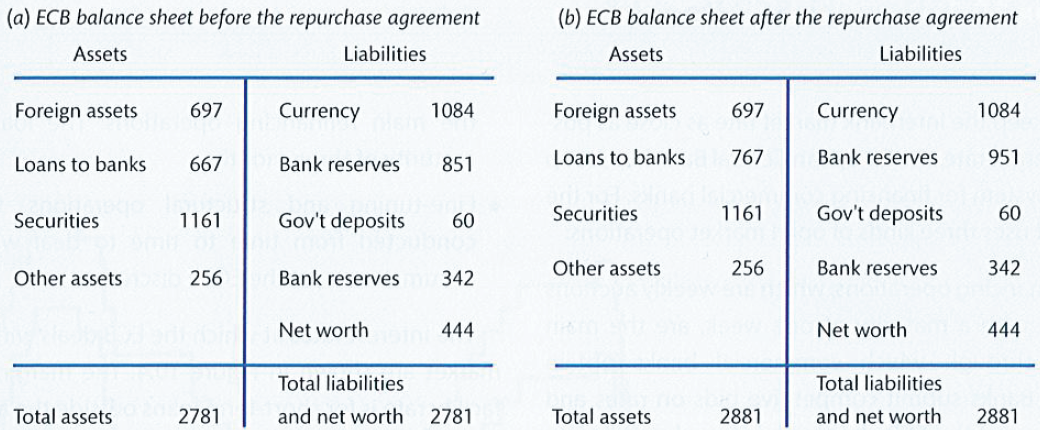
\includegraphics[trim=0 00 0 00,clip,width=0.6\textwidth]{FIGURES/5_CB_balance_sheet_OMO}
	%} 	
	%[trim=left bottom right top
\end{figure}
%\vspace{-2mm}
%\begin{minipage}{0.5\columnwidth}
%\tiny	
%\textbf{Source.} Burda and Wyplosz (2017), Figure 14.1.\\
%\end{minipage}
\end{center}

\end{frame}

\begin{frame}{Impulse response functions --- C, N}

  Transitory TFP shock: $\varepsilon$ rises from 0 to 0.1 ($=\sigma_\epsilon$) at $t=2$ and is at 0 afterwards:
\begin{center}
%{\small
%Figure. 
%}
\vspace{-5mm}
\begin{figure}[h!]
  \subfigure{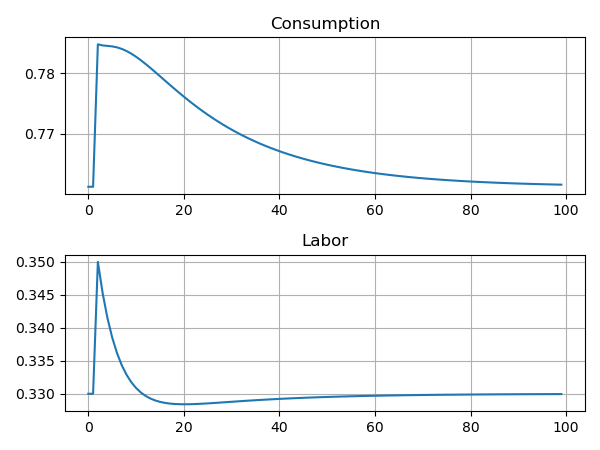
\includegraphics[trim=0 0 0 0,clip,width=0.9\textwidth]{FIGURES/irf_c_l.png}
	}      
	%\subfigure{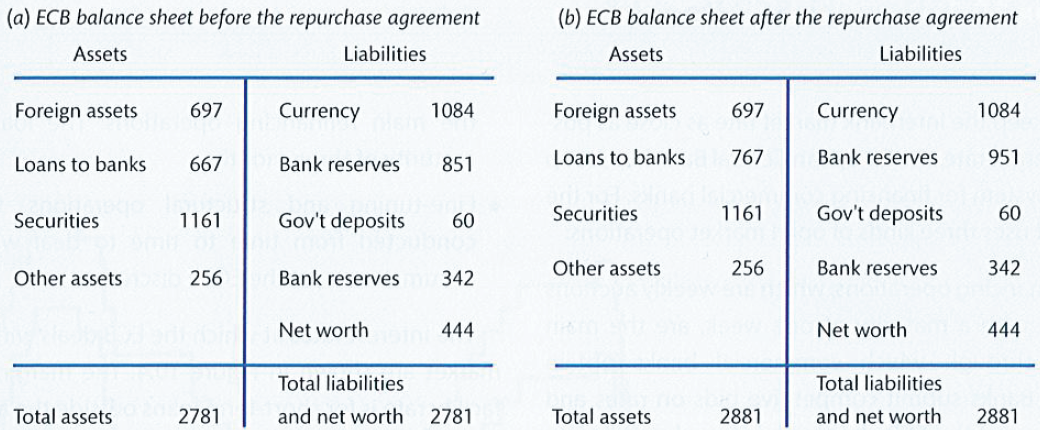
\includegraphics[trim=0 00 0 00,clip,width=0.6\textwidth]{FIGURES/5_CB_balance_sheet_OMO}
	%} 	
	%[trim=left bottom right top
\end{figure}
%\vspace{-2mm}
%\begin{minipage}{0.5\columnwidth}
%\tiny	
%\textbf{Source.} Burda and Wyplosz (2017), Figure 14.1.\\
%\end{minipage}
\end{center}

\end{frame}

\begin{frame}{Impulse response functions --- I, K}

  Transitory productivity shock: $\epsilon$ rises from 0 to $\sigma_\epsilon$ at $t=2$ and is at 0 afterwards:
\begin{center}
%{\small
%Figure. 
%}
\vspace{-5mm}
\begin{figure}[h!]
  \subfigure{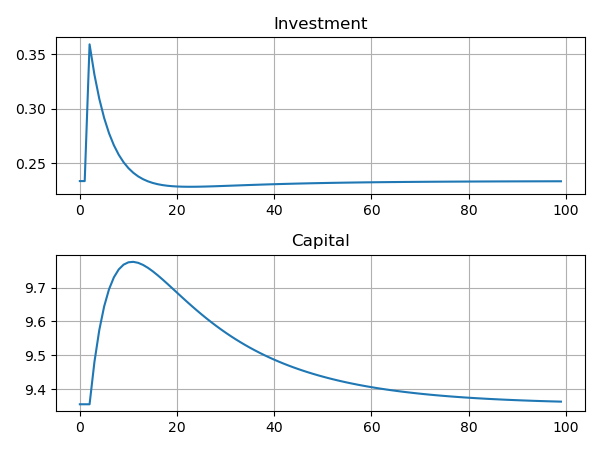
\includegraphics[trim=0 0 0 0,clip,width=0.9\textwidth]{FIGURES/irf_i_k.png}
	}      
	%\subfigure{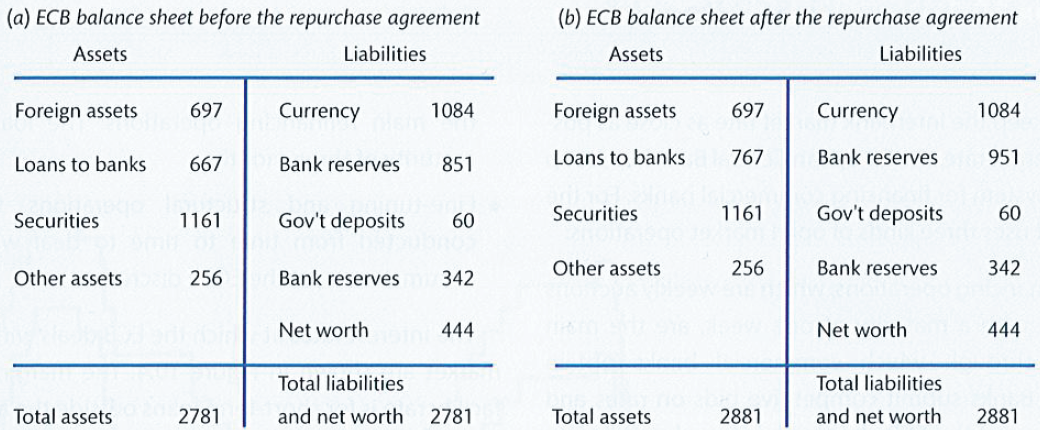
\includegraphics[trim=0 00 0 00,clip,width=0.6\textwidth]{FIGURES/5_CB_balance_sheet_OMO}
	%} 	
	%[trim=left bottom right top
\end{figure}
%\vspace{-2mm}
%\begin{minipage}{0.5\columnwidth}
%\tiny	
%\textbf{Source.} Burda and Wyplosz (2017), Figure 14.1.\\
%\end{minipage}
\end{center}

\end{frame}

\begin{frame}{Transitory vs. permanent productivity shock}

  Transitory shock (blue) -- as before; \\ \textbf{Permanent, anticipated shock} (orange) -- $\varepsilon_t$ constant for $t \geq 2$, such that $A_{ss}$ is 0.1 in new s.s.:
\begin{center}
%{\small
%Figure. 
%}
\vspace{-5mm}
\begin{figure}[h!]
  \subfigure{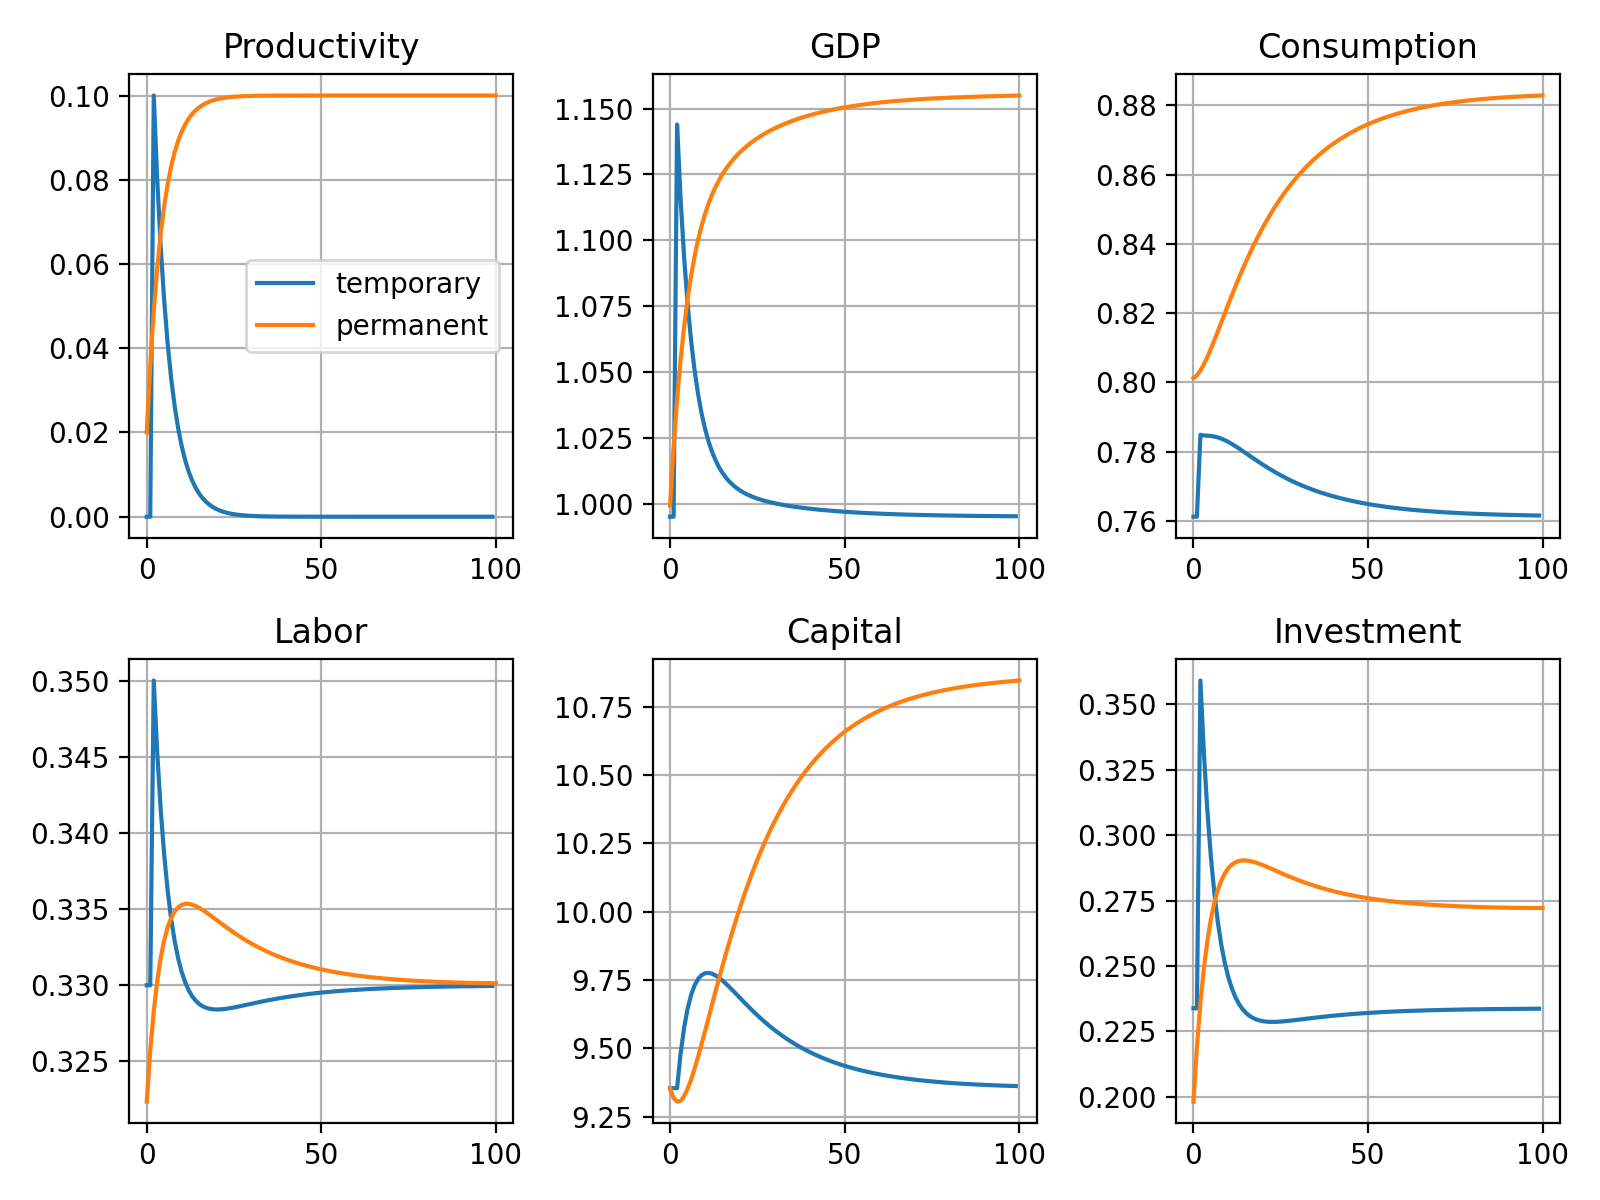
\includegraphics[trim=0 0 0 0,clip,width=0.85\textwidth]{FIGURES/perm_temp_lowsigma.png}
	}      
	%\subfigure{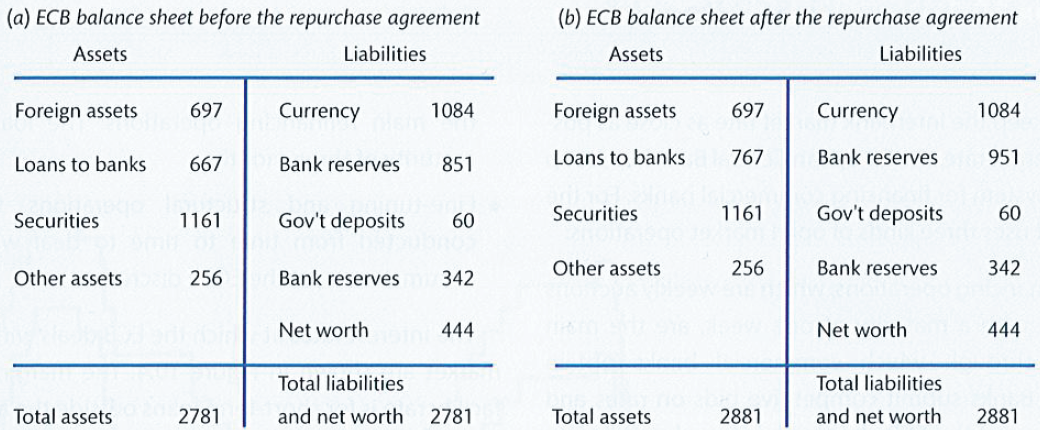
\includegraphics[trim=0 00 0 00,clip,width=0.6\textwidth]{FIGURES/5_CB_balance_sheet_OMO}
	%} 	
	%[trim=left bottom right top
\end{figure}
%\vspace{-2mm}
%\begin{minipage}{0.5\columnwidth}
%\tiny	
%\textbf{Source.} Burda and Wyplosz (2017), Figure 14.1.\\
%\end{minipage}
\end{center}
%
\end{frame}

\section{Social planning vs. equilibrium}

\begin{frame}
\frametitle{Outline}
\tableofcontents[currentsection]
\end{frame}

\begin{frame}{Social planner's problem}

\begin{mytemize}
\item The Social Planner
\begin{mytemize}
\item A fictional entity used to  to talk about optimal outcomes
\item Is \tb{benevolent} \rarr maximizes utility of representative household
\item Instead of optimizing w.r.t. prices, can reallocate goods between agents with no transaction cost 
  \rarr prices omitted from optimality analysis
\end{mytemize}
\item  The Social planner problem $\leftrightarrow$ finding optimal allocations:
\begin{mytemize}
\item Maximize a welfare criterion (benevolent \rarr HH utility)
\item ...subject to resource constraints -- physical constraints of economy
\end{mytemize}
\end{mytemize}


\end{frame}
%---FRAME------------------------------------------------------------------------------

\begin{frame}{Social Planner Optimization}

\begin{align*}
\max_{ C_t, N_t, K_{t+1} } E_0 \sum_{t=0}^{\infty} \beta^t  (u(C_t)+v(1-N_t))
\end{align*}
subject to a sequence of \tb{resource constraints}:
\begin{align*}
C_t + K_{t+1}-(1-\delta)K_t = A_t F(K_t,N_t) 
\end{align*}
FOCs of the Lagrangian with multipliers $\{\lambda_t\}$:
\begin{align*}
&\frac{\partial \mathcal{L}}{C_t} &= 0: \ \   & u'(C_t) -\lambda_t = 0\\
&\frac{\partial \mathcal{L}}{\partial N_t} &= 0: \ \   &-v'(1-N_t)+\lambda_t A_t F'_N(K_t,N_t)=0\\
&\frac{\partial \mathcal{L}}{\partial K_{t+1}} &= 0: \   &-\lambda_t  +\beta E_t[\lambda_{t+1}(A_{t+1}F'_K(K_{t+1},N_{t+1})+1-\delta)]=0 \\
\end{align*}

\end{frame}
%---FRAME------------------------------------------------------------------------------
\begin{frame}{Optimal allocations}
  \tb{Efficient allocation} then satisfies the system:
\begin{align*}
\frac{v'(1-N_t)}{u'(C_t)}&= A_t F'_N(K_t,N_t) \nonumber\\
u'(C_t) &= \beta E_t [u'(C_{t+1})(A_{t+1} F'_K(K_{t+1},N_{t+1})+1-\delta)] \\
C_t+K_{t+1}-(1-\delta)K_{t} &= A_t F(K_t,N_t) \nonumber \\
\ln A_t &= \rho \ln A_{t-1} + \varepsilon_t
\end{align*}
...which also gave the \tr{equilibrium}! \rarr \tb{equilibrium is optimal} \\
\vfill
\tms{This is a particular case of First Welfare Theorem that you will see in microeconomics} 
\vfill
The social planner \textbf{does not need prices} to achieve the equilibrium allocation
\end{frame}


\section{Capital adjustment cost}
\begin{frame}
\frametitle{Outline}
\tableofcontents[currentsection]
\end{frame}

%\begin{frame}{Investment impulse responses: model vs. data}
%  Investment is too ``jumpy'' in the baseline RBC w.r.t. data \\
%  \vfill
%  \rarr \tb{capital adjustment costs} introduced to model inertia.
%  \begin{figure}
%     \centering
%     \begin{subfigure}[b]{0.46\textwidth}
%         \centering
%		 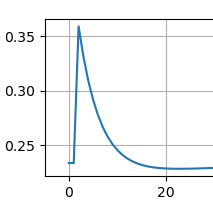
\includegraphics[width=\linewidth]{FIGURES/irf_i}
%		 \caption{Model IRF}
%     \end{subfigure}
%      \hfill
%     \begin{subfigure}[b]{0.52\textwidth}
%         \centering
%		 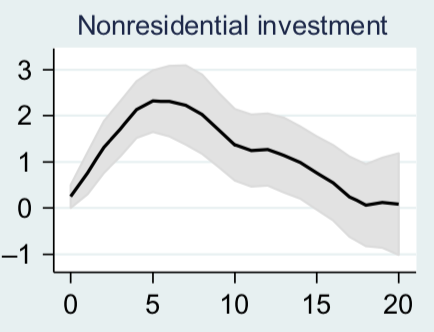
\includegraphics[width=\textwidth]{FIGURES/investment_VAR.png}
%		 \caption{Empirical IRF (Ramey, 2016)}
%     \end{subfigure}
%	 \caption{Investment reaction to transitory productivity shock.}
%\end{figure}
%\end{frame}
\begin{frame}{Capital adjustment cost}
    Most popular ``add-on'' to the RBC model \\ \vfill
    Makes investment more realistic: a more gradual response to TFP shocks \\ \vfill
    Modelling assumption: investment bears a \textbf{physical cost} \rarr some of the capital is lost in process
\end{frame}

\begin{frame}{Capital law of motion with adjustment costs}
  A new law of motion for capital: 
$$
K_{t+1}=I_{t}\textcolor{purple}{-\frac{\phi}{2}\left(\frac{I_{t}}{K_{t}}-\delta\right)^{2} K_{t}}+(1-\delta) K_{t}
$$
If $\phi>0$, then doing investment \textbf{above or below} steady state level (recall: in steady state $I_{ss}=\delta K_{ss}$ ) results in a cost  \\ \vfill Quadratic function: marginal cost increases as investment gets further from s.s. \\ \vfill \rarr Even if it is optimal increase capital stock significantly, the household will do it \textbf{in small steps}
\end{frame}

\begin{frame}{Household problem}
  New household problem, with functions chosen as before:
  $$
\begin{gathered}
\max_{C_{t}, I_{t}, N_{t}, K_{t+1}, B_{t+1}} E_{0} \sum_{t=0}^{\infty} \beta^{t}(u(C_t) + v(1-N_t)) \\
\text { s.t. } \quad
C_{t}+I_{t}+B_{t+1} =  w_{t} N_{t}+R_{t} K_{t}+\left(1+r_{t-1}\right) B_{t} +\Pi_{t}\\
K_{t+1}=I_{t}\textcolor{purple}{-\frac{\phi}{2}\left(\frac{I_{t}}{K_{t}}-\delta\right)^{2} K_{t}}+(1-\delta) K_{t}
\end{gathered}
$$
Two novelties:
\begin{mynumerate}
\item Two constraints, not one
\item Investment used as a choice variable ($K_{t+1}$ was chosen directly before)
\end{mynumerate}
\end{frame}

\begin{frame}{Household problem -- solution}
A Lagrangian with two constraints \rarr two multipliers, $\lambda$ and $\mu$:
\begin{align*}
\mathcal{L}=E_{0} \sum_{t=0}^{\infty} &\beta^{t}[u(C_t) + v(1-N_t) \\
&+\lambda_{t}(w_{t} N_{t}+R_{t} K_{t}+\Pi_{t}+\left(1+r_{t-1}\right) B_{t}-C_{t}-I_{t}-B_{t+1}) \\
&+\mu_{t}(I_{t}\textcolor{purple}{-\frac{\phi}{2}(\frac{I_{t}}{K_{t}}-\delta)^{2} K_{t}}+(1-\delta) K_{t}-K_{t+1})]
\end{align*}
\end{frame}

\begin{frame}{Household problem -- solution}
The new first order conditions are \tms{(obtain them yourself for training)}:
\begin{align*}
\frac{\partial \mathcal{L}}{\partial I_{t}}=0 &\Leftrightarrow \lambda_{t}=\mu_{t}(1-\phi(\frac{I_{t}}{K_{t}}-\delta)) \\
\frac{\partial \mathcal{L}}{\partial K_{t+1}}=0 &\Leftrightarrow  \\ \mu_{t}=\beta E_{t}[&R_{t+1} \lambda_{t+1}-\mu_{t+1} \frac{\phi}{2}(\frac{I_{t+1}}{K_{t+1}}-\delta)^{2} \\
&+\mu_{t+1} \phi(\frac{I_{t+1}}{K_{t+1}}-\delta) \frac{I_{t+1}}{K_{t+1}}+\mu_{t+1}(1-\delta)] 
\end{align*}

\end{frame}

\begin{frame}{Tobin's q is back}

  We define \tb{$q_{t} \equiv \frac{\mu_{t}}{\lambda_{t}}$} 
\begin{mytemize}
\item	$\mu_{t}$ -- marginal utility of additional capital installed
\item $\lambda_{t}$ -- marginal utility of consumption 
\item The ratio $q_t$ -- how much consumption you would give up to have some extra future capital
\item At the same time, \textbf{the price of capital good is 1}, same as consumption good
\item[\rarr] $q_t$ is theoretical \tb{Tobin's q} -- ratio of willingness-to-pay to price of physical capital goods
\end{mytemize}
\vfill
The FOC $\frac{\partial \mathcal{L}}{\partial I_{t}}=0$ can be re-written: 
$
q_{t}=\left(1-\phi\left(\frac{I_{t}}{K_{t}}-\delta\right)\right)^{-1} 
$ \\
\vfill
\rarr positive association between $I_t$ and $q_t$: $I(\underset{+}{q_t},\dots)$ \\
\vfill
  Main implication for equilibrium: additional \tb{inertia} in investment.
\end{frame}

\begin{frame}{Impulse responses with various capital adjustment costs}
  \vspace{-0.1cm}
  \begin{figure}[ht]
	\centering
	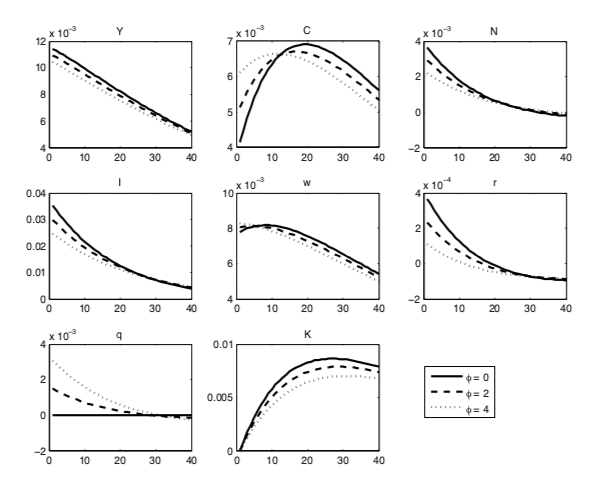
\includegraphics[width = 0.92\linewidth]{FIGURES/Adjust_cost_IRF_EricSims}
	\caption{Response to TFP shock under different magnitudes of cap. adj. cost }
  \end{figure}
\end{frame}

%\begin{frame}{Alternative specifications}
%  The form of adjustment cost is the simplest one; investment less reactive, but still not ``hump-shaped'' as in empirical IRF.
%
%  Several other options exist:
%  \begin{enumerate}
%	\item Specified in HH budget constraint directly:
%	  \begin{align*}
%		C_t + I_t + B_{t+1} &= w_t L_t + R_t K_t \textcolor{purple}{- \frac{1}{2} \frac{I^2_t}{K_t}} \\
%		\text{or} \quad	C_t + I_t + B_{t+1} &= w_t L_t + R_t K_t \textcolor{purple}{- \Phi(K_{t+1} - K_t)}, \ \text{with} \ \Phi', \Phi''>0 
%	  \end{align*}
%	\item Specified in law of motion of capital, but w.r.t. investment variable only -- \tb{investment adjustment cost}:
%$$
%K_{t+1}=\textcolor{purple}{\left[1-\frac{\phi}{2}\left(\frac{I_{t}}{I_{t-1}}-1\right)^2 \right]} I_{t}+(1-\delta) K_{t}
%$$
%Here, investment can be called both a \tm{state} and a \tm{control}. \\
%\vfill
%Investment adjustment cost is known to produce hump-shaped reactions of investment to productivity shocks.
%  \end{enumerate}
%\end{frame}
%
%
%\begin{frame}{Investment adjustment cost -- impulse responses}
%  \begin{figure}[ht]
%	\centering
%	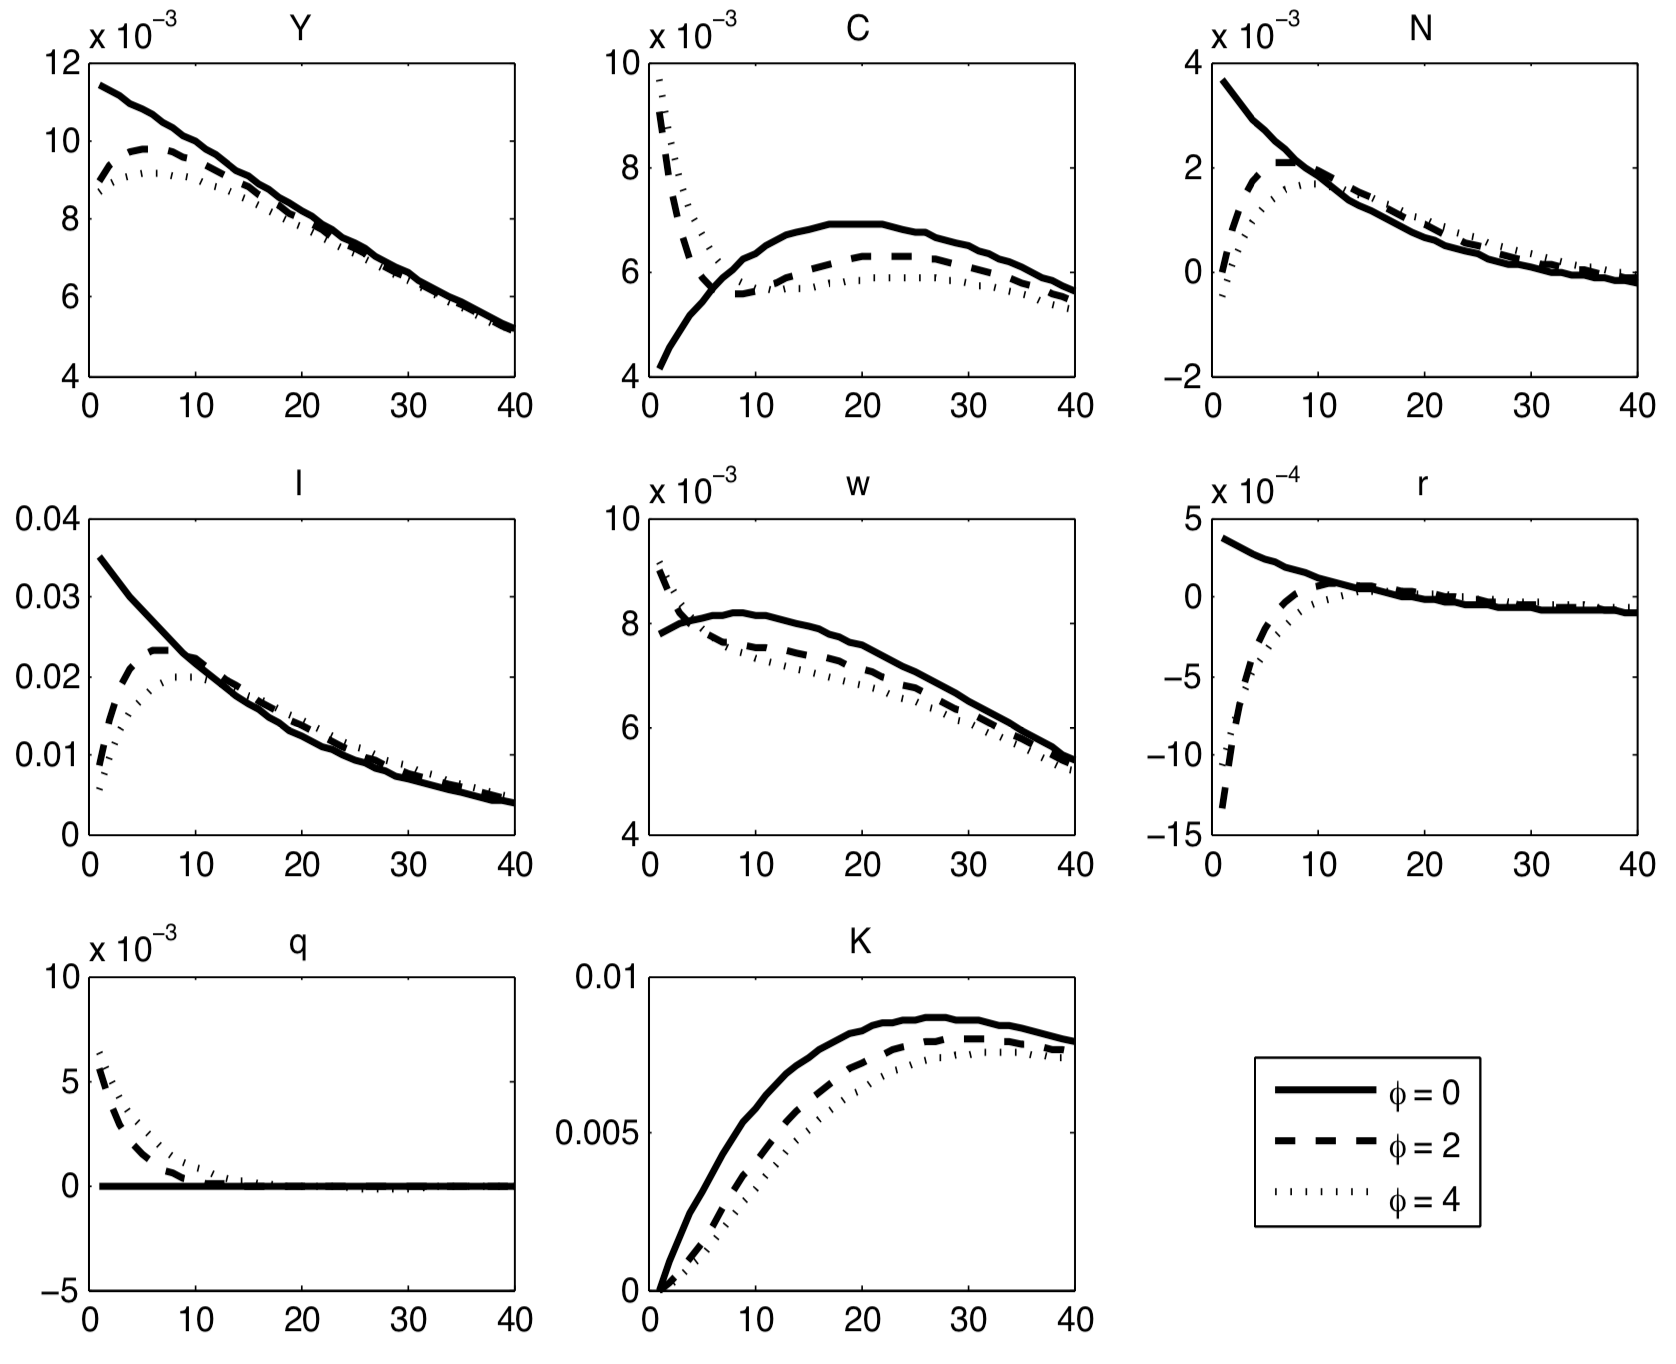
\includegraphics[width=0.95\textwidth]{FIGURES/inv_adj_cost_IRF_EricSims}
%  \end{figure}
%\end{frame}


\end{document}
